\ChapterImageStar[cap:pmv]{Producto Mínimo Viable}{./images/fondo.png}\label{cap:pmv}
\mbox{}\\
\section{Estructura del proyecto}
\noindent
La figura~\ref{fig:estructura-proyecto} detalla la estructura del proyecto
\begin{figure}[H]
    \centering
    \begin{minipage}{0.48\textwidth}
        \centering
        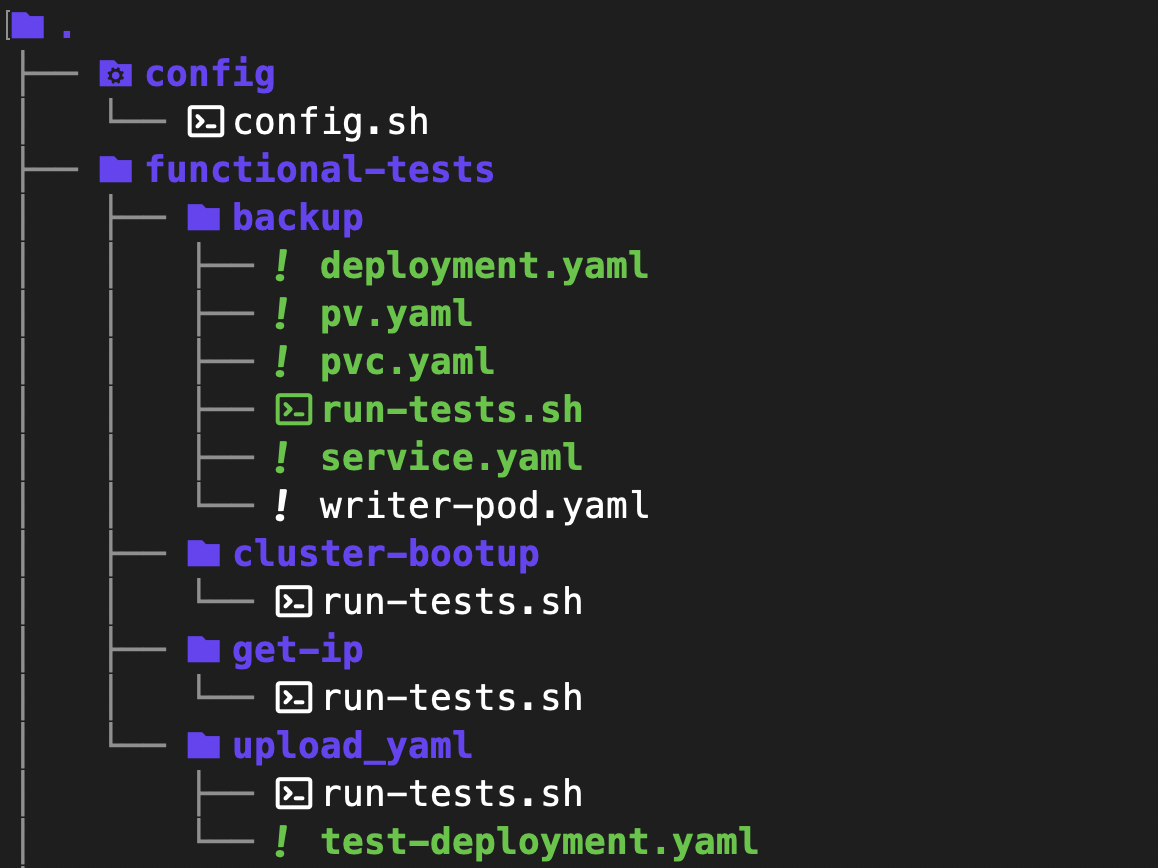
\includegraphics[scale=0.35]{tablas-images/cp6/src/tree-1.png}
        \subcaption{Parte 1}\label{fig:estructura-proyecto-1}
    \end{minipage}
    \hfill
    \begin{minipage}{0.48\textwidth}
        \centering
        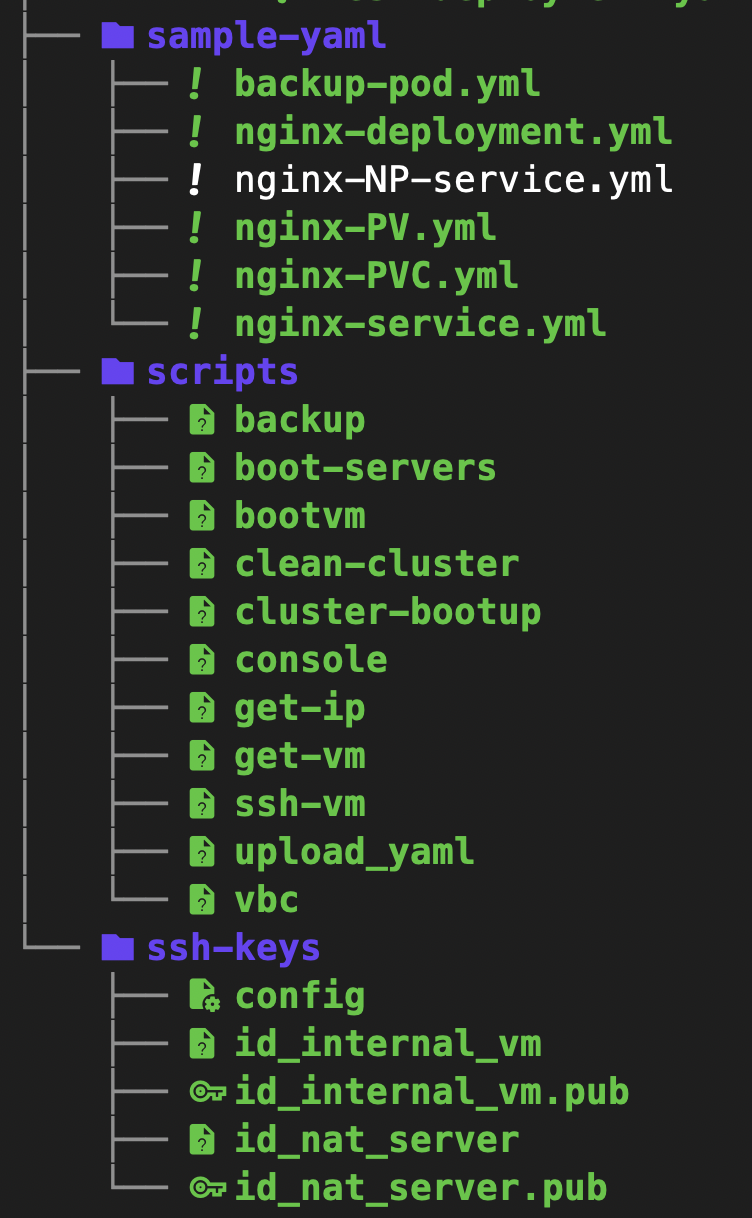
\includegraphics[scale=0.35]{tablas-images/cp6/src/tree-2.png}
        \subcaption{Parte 2}\label{fig:estructura-proyecto-2}
    \end{minipage}
    \caption{Estructura del proyecto}\label{fig:estructura-proyecto}
\end{figure}

\section{Código fuente}\label{sec:automatizacion-scripts}
\noindent
El código fuente del sistema, desarrollado en el lenguaje Bash, está disponible en el repositorio de GitHub \href{https://github.com/AariazP/TG-VBC.git}{\texttt{TG-VBC}} en la rama \texttt{scripted-solution}. Este repositorio contiene scripts para la automatización de tareas en la infraestructura de virtualización basada en contenedores, incluyendo la configuración de nodos, despliegue de \VM\ y configuración de Kubernetes. 

\subsection{Config}
\noindent
Este paquete contiene scripts de configuración y utilidades para la gestión de máquinas virtuales en un entorno XCP-ng.
%=========================CONFIG=========================
\subsubsection{Config.sh}
\noindent
El siguiente script en \textit{bash} tiene como finalidad modificar la tabla de enrutamiento del sistema mediante la adición de una ruta estática. 
De esta manera, se define un camino específico para que los paquetes dirigidos a la red \texttt{192.168.100.0/24} sean encaminados a través de la 
puerta de enlace \texttt{172.30.29.2}, utilizando la interfaz de red \texttt{xenbr0}. 
Este tipo de configuración es común en entornos de virtualización como Xen o XCP-ng, donde los bridges de red permiten interconectar  máquinas virtuales con la red física.

\begin{minted}[frame=lines,
    fontsize=\scriptsize,
    breaklines]{bash}
#!/bin/bash

# Agrega una ruta estática a la tabla de enrutamiento del sistema.
# En este caso, se está indicando que para llegar a la red 192.168.100.0/24 
# (es decir, todas las IP desde 192.168.100.1 hasta 192.168.100.254 con máscara /24),
# el tráfico debe enviarse a través de la puerta de enlace 172.30.29.2,
# utilizando la interfaz de red xenbr0 (un bridge, normalmente en entornos con Xen o XCP-ng).
sudo ip route add 192.168.100.0/24 via 172.30.29.2 dev xenbr0
\end{minted}

%=========================functional-test/backup=========================
\subsection{functional-test/backup}
\noindent
La siguiente sección presenta los distintos manifiestos y scripts que conforman la estrategia de creación de respaldo en Kubernetes. Cada archivo cumple un rol específico dentro del despliegue, desde la definición del pod y sus volúmenes. A continuación, se describen brevemente los archivos incluidos en este paquete:
\subsubsection{deployment.yaml}
\noindent
El siguiente manifiesto en formato \texttt{YAML} define un recurso de tipo \texttt{Deployment} en Kubernetes para la aplicación \texttt{nginx}. Este despliegue solicita que exista al menos una réplica en ejecución, gestionada automáticamente por el controlador de Kubernetes. Además, se especifican etiquetas para la selección de pods, la imagen utilizada del contenedor, los puertos expuestos y un volumen persistente que se monta en el directorio \texttt{/usr/share/nginx/html}, el cual permite servir archivos estáticos de manera persistente.

\begin{minted}[frame=lines,
    fontsize=\scriptsize,
    breaklines]{yaml}
apiVersion: apps/v1             # Versión de la API de Kubernetes utilizada para el recurso
kind: Deployment                # Tipo de recurso: Deployment (gestiona pods y réplicas)
metadata:
  name: nginx-deployment        # Nombre asignado al Deployment
spec:
  replicas: 1                   # Número de réplicas del pod
  selector:
    matchLabels:
      app: nginx                # Selector para identificar los pods asociados
  template:                     # Plantilla que define cómo serán los pods
    metadata:
      labels:
        app: nginx              # Etiquetas aplicadas al pod
    spec:
      containers:
        - name: nginx           # Nombre del contenedor
          image: nginx:stable   # Imagen de Docker utilizada
          ports:
            - containerPort: 80 # Puerto expuesto por el contenedor (HTTP)
          volumeMounts:
            - name: nginx-storage
              mountPath: /usr/share/nginx/html  # Montaje del volumen para archivos estáticos
      volumes:
        - name: nginx-storage
          persistentVolumeClaim:
            claimName: nginx-pvc # Reclamo de volumen persistente asociado
\end{minted}

\subsubsection{pv.yaml}
\noindent
El siguiente manifiesto en \texttt{YAML} define un recurso de tipo \texttt{PersistentVolume} (PV) en Kubernetes, 
el cual representa una pieza de almacenamiento en el clúster que puede ser reclamada por los pods mediante 
un \texttt{PersistentVolumeClaim} (PVC). En este caso, el volumen tiene una capacidad de \texttt{1Gi}, con 
modo de acceso \texttt{ReadWriteOnce}, lo que significa que puede ser montado en modo lectura y escritura por 
un único nodo al mismo tiempo. La configuración utiliza un \texttt{hostPath}, lo que enlaza el volumen a una 
ruta del sistema de archivos del nodo anfitrión (\texttt{/mnt/data/nginx}).

\begin{minted}[frame=lines,
    fontsize=\scriptsize,
    breaklines]{yaml}
apiVersion: v1                # Versión de la API de Kubernetes para recursos básicos
kind: PersistentVolume         # Tipo de recurso: PersistentVolume (PV)
metadata:
  name: nginx-pv               # Nombre asignado al volumen persistente
spec:
  capacity:
    storage: 1Gi               # Capacidad de almacenamiento asignada al volumen
  accessModes:
    - ReadWriteOnce            # Permite acceso de lectura/escritura desde un solo nodo
  hostPath:                    # Define un path físico en el nodo (útil en pruebas locales)
    path: /mnt/data/nginx      # Ruta en el sistema de archivos del nodo donde se almacena el volumen
\end{minted}
\subsubsection{service.yaml}
\noindent
Este archivo YAML define un recurso \texttt{PersistentVolumeClaim (PVC)}, que permite a los pods solicitar almacenamiento persistente de acuerdo con lo especificado en un \texttt{PersistentVolume (PV)} previamente configurado. En este caso, el PVC solicita \texttt{1~GiB} de almacenamiento con modo de acceso \texttt{ReadWriteOnce}, lo que significa que solo un nodo podrá montar el volumen en modo lectura y escritura de manera simultánea. El PVC funciona como una capa intermedia entre los pods y el PV, desacoplando la aplicación de los detalles específicos de la infraestructura de almacenamiento.

\begin{minted}[frame=lines,
    fontsize=\scriptsize,
    breaklines]{yaml}
apiVersion: v1
kind: PersistentVolumeClaim
metadata:
  name: nginx-pvc
spec:
  accessModes:
    - ReadWriteOnce
  resources:
    requests:
      storage: 1Gi
\end{minted}
\subsubsection{writer-pod.yaml}
\noindent
Este manifiesto define un \texttt{Pod} denominado \texttt{writer-pod}, cuyo propósito es servir como contenedor de prueba para validar la persistencia de datos en Kubernetes. El pod utiliza la imagen ligera \texttt{busybox}, ejecutándose en segundo plano mediante el comando \texttt{sleep} para mantenerse activo. Además, monta un volumen persistente a través del \texttt{PersistentVolumeClaim} \texttt{nginx-pvc}, asignando la ruta interna \texttt{/data}. De esta manera, cualquier dato escrito en dicho directorio dentro del pod se almacenará en el volumen persistente, permitiendo comprobar la correcta configuración de la capa de almacenamiento.

\begin{minted}[frame=lines,
    fontsize=\scriptsize,
    breaklines]{yaml}
apiVersion: v1
kind: Pod
metadata:
  name: writer-pod
spec:
  containers:
    - name: writer
      image: busybox
      command: [ "sleep", "3600" ]  # mantiene el pod activo
      volumeMounts:
        - mountPath: /data          # directorio donde se montará el PVC
          name: nginx-storage
  volumes:
    - name: nginx-storage
      persistentVolumeClaim:
        claimName: nginx-pvc        # vínculo al PVC previamente creado
\end{minted}

\subsubsection{run-tests.sh}
\noindent
Este script en bash automatiza el proceso de validación funcional de un entorno de Kubernetes desplegado en un clúster virtual. Primero realiza el arranque de las máquinas virtuales del clúster y carga los archivos \texttt{.yaml} necesarios para el despliegue de recursos (deployment, volúmenes persistentes, servicio y un pod de prueba denominado \texttt{writer-pod}). Luego, espera hasta que dicho pod se encuentre en estado \texttt{Running}, tras lo cual se ejecutan comandos dentro de él para crear archivos de prueba en el volumen asociado. Finalmente, el script realiza respaldos tanto a nivel del volumen persistente \texttt{(PVC)} como directamente desde el pod, verificando la integración de la capa de almacenamiento con las aplicaciones en ejecución.

\begin{minted}[frame=lines,
    fontsize=\scriptsize,
    breaklines]{bash}
#!/bin/bash

# Muestra mensaje de inicio de arranque de VMs del clúster
echo "======= Booting vms ======="
cluster-bootup -m 1 -w 2   # Inicia 1 master y 2 workers

# Sube los manifiestos .yaml al nodo master
echo "====== Uploadindg .yaml files ========"
upload_yaml master1 deployment.yaml
upload_yaml master1 pvc.yaml
upload_yaml master1 pv.yaml
upload_yaml master1 service.yaml
upload_yaml master1 writer-pod.yaml

# Verifica el estado del pod hasta que esté en Running
echo "======= modyfing files ========"
while ! ssh-vm -r master1 -c "kubectl get pod/writer-pod" | grep -q Running 
do
   sleep 1
done

# Escribe un archivo de prueba en el volumen persistente
ssh-vm -r master1 -c "kubectl exec writer-pod -- sh -c 'echo functional test for backup > /data/dummy_file.txt'"

# Realiza respaldo del PVC asociado
echo "====== backing up for pvc ======="
backup nginx-pvc

# Escribe un archivo de prueba directamente en el pod
echo "====== backing up for pod ======="
ssh-vm -r master1 -c "kubectl exec writer-pod -- sh -c 'echo functional test for backup in a pod > /data/dummy_file_pod.txt'"

# Realiza respaldo a nivel de pod, copiando datos desde /data
backup -p writer-pod:/data
\end{minted}



%=========================functional-test/cluster-bootup=========================

\subsection{functional-test/cluster-bootup}
\noindent

\subsubsection{run-tests.sh}
\noindent
Este script en \texttt{bash} implementa un conjunto de pruebas funcionales automatizadas para verificar la correcta creación de clústeres virtuales mediante el uso de la herramienta \texttt{cluster-bootup}. Se evalúan tres configuraciones distintas: un clúster con un maestro y un trabajador, un clúster con dos maestros y un trabajador, y finalmente una variante que además incluye un servidor \texttt{NAT-Backup}. El script compara los resultados esperados con los obtenidos tras el despliegue de las máquinas virtuales, contabilizando las pruebas superadas y limpiando el clúster al finalizar cada verificación. De esta forma, se garantiza la reproducibilidad y consistencia en los entornos de prueba.  

\begin{minted}[frame=lines,
    fontsize=\scriptsize,
    breaklines]{bash}
#!/bin/bash

# Contador de pruebas exitosas
SUCCEDEED_TESTS=0

# Función de verificación: compara valores esperados con resultados
check(){
     echo +++++++++++++++++strings+++++++++++++++++++++++++
     echo $2
     echo $3
     if [[ "$2" == "$3" ]]
     then
        echo "Test for $1 succedeed"
        SUCCEDEED_TESTS=$(( $SUCCEDEED_TESTS + 1 ))
        return 0
     fi

     echo "Test for $1 failed"
     return 1
}

# ===== Primera prueba: 1 master, 1 worker =====
export EXPECTED_RESULT=" master1 NAT-Master worker1"
cluster-bootup -m 1 -w 1
export RESULT=$( get-vm | sort | tr -d '\n')
check  "1 master 1 worker" "$EXPECTED_RESULT" "$RESULT"
clean-cluster -y

# ===== Segunda prueba: 2 masters, 1 worker =====
export EXPECTED_RESULT=" load-balancer1 master1 master2 NAT-Master worker1"
cluster-bootup -m 2 -w 1
export RESULT=$( get-vm | sort | tr -d '\n')
check  "2 master 1 worker" "$EXPECTED_RESULT" "$RESULT"
clean-cluster -y

# ===== Tercera prueba: 2 masters, 1 worker, 1 NAT Backup =====
export EXPECTED_RESULT=" load-balancer1 master1 master2 NAT-Backup NAT-Master worker1"
cluster-bootup -m 2 -w 1 -b
export RESULT=$( get-vm | sort | tr -d '\n')
check  "2 master 1 worker 1 NAT Backup" "$EXPECTED_RESULT" "$RESULT"
clean-cluster -y

# Reporte final de pruebas
echo "${SUCCEDEED_TESTS}/3 tests succeeded"
\end{minted}


%=========================functional-test/get-ip=========================

\subsection{functional-test/get-ip}
\noindent

\subsubsection{run-tests.sh}
\noindent
Este script en \texttt{bash} realiza una serie de pruebas para validar la correcta creación de un clúster con dos nodos maestros, un nodo trabajador, un balanceador de carga y un servidor \texttt{NAT-Backup}. Tras ejecutar el despliegue mediante la función \texttt{cluster-bootup}, el script verifica que cada máquina virtual reciba la dirección IP correspondiente a su rol: los maestros, el trabajador y el balanceador de carga dentro de la red \texttt{192.x.x.x}, mientras que los servidores NAT deben ubicarse en la subred \texttt{172.x.x.x}. Cada prueba exitosa incrementa un contador, y al final se presenta un resumen del total de pruebas superadas.  

\begin{minted}[frame=lines,
    fontsize=\scriptsize,
    breaklines]{bash}
#!/bin/bash

# Inicia el clúster con:
# - 1 worker
# - 2 masters
# - servidor NAT de respaldo (-b)
cluster-bootup -w 1 -m 2 -b

# Breve pausa para dar tiempo a que arranquen las VMs
sleep 2

# Contador de pruebas exitosas
SUCCESS_TEST_COUNT=0

# Verificación de IPs según el rol de cada VM
get-ip master1 | grep 192 && echo "Test for master succedeed" \
  && SUCCESS_TEST_COUNT=$(( $SUCCESS_TEST_COUNT + 1 ))

get-ip worker1 | grep 192 && echo "Test for worker succedeed" \
  && SUCCESS_TEST_COUNT=$(( $SUCCESS_TEST_COUNT + 1 ))

get-ip load-balancer | grep 192 && echo "Test for load-balancer succedeed" \
  && SUCCESS_TEST_COUNT=$(( $SUCCESS_TEST_COUNT + 1 ))

get-ip NAT-Master | grep 172 && echo "Test for NAT-Master succedeed" \
  && SUCCESS_TEST_COUNT=$(( $SUCCESS_TEST_COUNT + 1 ))

get-ip NAT-Backup | grep 172 && echo "Test for NAT-Backup succedeed" \
  && SUCCESS_TEST_COUNT=$(( $SUCCESS_TEST_COUNT + 1 ))

# Resultado final de las pruebas
echo "$SUCCESS_TEST_COUNT/5 tests succedeed"
\end{minted}



%=========================functional-test/aplicar-yml=========================/

\subsection{functional-test/upload-yaml}

\subsubsection{test-deployment.yaml}
\noindent
Este archivo en formato \texttt{YAML} define un objeto de tipo \texttt{Deployment} en Kubernetes para desplegar una instancia de Nginx. El despliegue crea un único pod (\texttt{replicas: 1}) que utiliza la imagen estable de Nginx y expone el puerto 80 para atender solicitudes HTTP. Además, mediante la sección \texttt{selector} y las etiquetas (\texttt{labels}), se asegura la asociación entre el \texttt{Deployment} y los pods que administra, garantizando que Kubernetes mantenga en ejecución la cantidad definida de réplicas.

\begin{minted}[frame=lines,
    fontsize=\scriptsize,
    breaklines]{yaml}

apiVersion: apps/v1
kind: Deployment
metadata:
  name: nginx-deployment
spec:
  replicas: 1
  selector:
    matchLabels:
      app: nginx
  template:
    metadata:
      labels:
        app: nginx
    spec:
      containers:
        - name: nginx
          image: nginx:stable
          ports:
            - containerPort: 80

\end{minted}


\subsubsection{run-tests.sh}
\noindent
Este script en \texttt{bash} realiza una prueba funcional básica sobre un clúster recién creado. Primero levanta la infraestructura mínima con un nodo maestro y un nodo trabajador. Luego, transfiere y aplica en el maestro un archivo \texttt{YAML} que define un despliegue de prueba (\texttt{test-deployment.yaml}). Finalmente, el script comprueba si el despliegue denominado \texttt{nginx-deployment} se encuentra en ejecución mediante el comando \texttt{kubectl get pods}. Si se detecta correctamente, se imprime un mensaje de éxito; en caso contrario, se muestra un mensaje de fallo.  

\begin{minted}[frame=lines,
    fontsize=\scriptsize,
    breaklines]{bash}

#!/bin/bash

# Levanta un clúster con:
# - 1 nodo master
# - 1 nodo worker
cluster-bootup -m 1 -w 1

# Sube y aplica el archivo YAML al nodo master1
upload_yaml master1 test-deployment.yaml

# Verifica que el pod asociado al despliegue "nginx-deployment" esté corriendo.
# Si aparece en la lista de pods, la prueba es exitosa, de lo contrario falla.
ssh-vm -r master1 -c "kubectl get pods" | grep -q nginx-deployment \
    && echo "Test succedeed" \
    || echo "Test failed"

\end{minted}






\subsection{sample-yaml}
\noindent

\subsubsection{backup-pod.yml}
\noindent
\begin{minted}[frame=lines,
    fontsize=\scriptsize,
    breaklines]{yaml}
apiVersion: v1
kind: Pod
metadata:
  name: backup-pod
spec:
  containers:
  - name: backup
    image: alpine
    command: [ "sleep", "3600" ]
    volumeMounts:
    - mountPath: /data
      name: app-data
  volumes:
  - name: app-data
    persistentVolumeClaim:
      claimName: your-pvc
\end{minted}

\subsubsection{nginx-deployment.yml}
Este manifiesto en \texttt{YAML} define un \texttt{Deployment} en Kubernetes llamado \texttt{nginx-deployment}, cuya función es desplegar y gestionar un conjunto de réplicas del servidor web Nginx. En este caso, se especifica que el despliegue debe mantener tres instancias (\texttt{replicas: 3}) del contenedor basado en la imagen \texttt{nginx:1.25}. Cada contenedor expone el puerto \texttt{80}, permitiendo servir tráfico HTTP. El uso de etiquetas (\texttt{app: nginx}) facilita la selección y organización de los recursos asociados a este despliegue.

\begin{minted}[frame=lines,
    fontsize=\scriptsize,
    breaklines]{yaml}
apiVersion: apps/v1
kind: Deployment
metadata:
  name: nginx-deployment
  labels:
    app: nginx
spec:
  replicas: 3
  selector:
    matchLabels:
      app: nginx
  template:
    metadata:
      labels:
        app: nginx
    spec:
      containers:
      - name: nginx
        image: nginx:1.25
        ports:
        - containerPort: 80
\end{minted}

\subsubsection{nginx-NP-service.yml}
Este manifiesto en \texttt{YAML} define un recurso \texttt{Service} de tipo \texttt{NodePort} en Kubernetes, llamado \texttt{nginx-nodeport}. Su objetivo es exponer las aplicaciones etiquetadas con \texttt{app: nginx} hacia el exterior del clúster, permitiendo el acceso al puerto \texttt{80} del contenedor a través del puerto \texttt{30080} en los nodos del clúster. De esta forma, cualquier petición dirigida al puerto \texttt{30080} de un nodo será redirigida al puerto interno \texttt{80} de los pods correspondientes, facilitando el acceso externo al servicio.

\begin{minted}[frame=lines,
    fontsize=\scriptsize,
    breaklines]{yaml}
apiVersion: v1
kind: Service
metadata:
  name: nginx-nodeport
spec:
  type: NodePort
  selector:
    app: nginx
  ports:
    - port: 80            
      targetPort: 80      
      nodePort: 30080     
\end{minted}

\subsubsection{nginx-PV.yml}
El siguiente manifiesto en \texttt{YAML} define un recurso \texttt{PersistentVolume} (PV) en Kubernetes, denominado \texttt{pv-sample}. Este volumen proporciona un almacenamiento de \texttt{1Gi} con modo de acceso \texttt{ReadWriteOnce}, lo cual permite que un único nodo lo monte en modo lectura y escritura. La política de recuperación establecida es \texttt{Retain}, lo que significa que los datos no serán eliminados automáticamente cuando el volumen quede liberado. Además, se especifica una clase de almacenamiento manual (\texttt{manual}) y un \texttt{hostPath} que apunta al directorio \texttt{/mnt/data} del nodo anfitrión, vinculando el almacenamiento físico del host con el clúster.

\begin{minted}[frame=lines,
    fontsize=\scriptsize,
    breaklines]{yaml}
apiVersion: v1
kind: PersistentVolume
metadata:
  name: pv-sample
spec:
  capacity:
    storage: 1Gi
  accessModes:
    - ReadWriteOnce
  persistentVolumeReclaimPolicy: Retain
  storageClassName: manual
  hostPath:
    path: "/mnt/data"
\end{minted}


\subsubsection{nginx-PVC.yml}
El recurso \texttt{PersistentVolumeClaim} (PVC) en Kubernetes actúa como una solicitud de almacenamiento por parte de una aplicación dentro del clúster. En este caso, el PVC denominado \texttt{pvc-sample} solicita un volumen con capacidad de \texttt{1Gi}, en modo de acceso \texttt{ReadWriteOnce}, lo cual permite que solo un nodo lo monte con permisos de lectura y escritura al mismo tiempo. Este reclamo hace uso de la clase de almacenamiento \texttt{manual}, lo que asegura su vinculación con el \texttt{PersistentVolume} previamente definido que comparte las mismas características.

\begin{minted}[frame=lines,
    fontsize=\scriptsize,
    breaklines]{yaml}
apiVersion: v1
kind: PersistentVolumeClaim
metadata:
  name: pvc-sample
spec:
  accessModes:
    - ReadWriteOnce
  storageClassName: manual
  resources:
    requests:
      storage: 1Gi
\end{minted}

\subsubsection{nginx-service.yml}
El recurso \texttt{Service} en Kubernetes permite exponer aplicaciones desplegadas dentro del clúster, asegurando una comunicación estable entre pods y otros componentes. En este caso, el servicio denominado \texttt{nginx-service} está configurado con el tipo \texttt{ClusterIP}, lo que significa que será accesible únicamente desde dentro del clúster. Su selector utiliza la etiqueta \texttt{app: nginx} para dirigir el tráfico hacia los pods gestionados por el \texttt{Deployment} de Nginx. El puerto expuesto es el \texttt{80}, el cual redirige al mismo \texttt{targetPort} dentro de los contenedores.

\begin{minted}[frame=lines,
    fontsize=\scriptsize,
    breaklines]{yaml}
apiVersion: v1
kind: Service
metadata:
  name: nginx-service
spec:
  selector:
    app: nginx
  ports:
    - protocol: TCP
      port: 80
      targetPort: 80
  type: ClusterIP
\end{minted}

\subsection{Scripts}

\subsection{backup.sh}
\noindent
\begin{minted}[frame=lines,
    fontsize=\scriptsize,
    breaklines]{bash}
#!/bin/bash

# ensures file cleanup after cancellation

trap "rm -f exporter_file.yaml" SIGINT

MODE="pvc"
TARGET=""
POD=""
FOLDER=""
while getopts "p:f:" opt; do
  case "$opt" in
    p) MODE="pod"; POD="$OPTARG" ;;     # backup from pod:path
    f) MODE="folder"; FOLDER="$OPTARG" ;; # backup from host path
  esac
done
shift $((OPTIND-1))

NODE="$( get-vm -a -n 1 master )"

PVC="$1"
DATE=$( date +%Y-%m-%d-%H-%M-%S-%s )

if [[ "$MODE" == "pvc" ]]; then
  # --- current PVC backup flow ---
  cat <<EOF > exporter_file.yaml
apiVersion: v1
kind: Pod
metadata:
  name: exporter
spec:
  containers:
  - name: exporter
    image: alpine
    command: ["sleep", "3600"]
    volumeMounts:
    - mountPath: /data
      name: export-pvc
  volumes:
  - name: export-pvc
    persistentVolumeClaim:
      claimName: ${PVC}
EOF

  upload_yaml ${NODE} exporter_file.yaml

  while [[ $(ssh-vm -r ${NODE} -c "kubectl get pod/exporter -o jsonpath='{.status.phase}'") != "Running" ]]; do
    sleep 1
  done
  FILENAME="/tmp/backup-${DATE}-pvc.tar"
  ssh-vm -r ${NODE} -c "kubectl cp exporter:/data ./backup-${DATE}"
  ssh-vm -r ${NODE} -c "kubectl delete pod/exporter"
  ssh-vm -r ${NODE} -c "tar -cvf ${FILENAME} ./backup-${DATE}"

elif [[ "$MODE" == "pod" ]]; then
  FILENAME="/tmp/backup-${DATE}-pod.tar"
  # --- backup arbitrary path from pod ---
  ssh-vm -r ${NODE} -c "kubectl cp ${POD} ./backup-${DATE}"
  ssh-vm -r ${NODE} -c "tar -cvf ${FILENAME} ./backup-${DATE}"

elif [[ "$MODE" == "folder" ]]; then
  FILENAME="/tmp/backup-${DATE}-node.tar"
  # --- backup arbitrary folder from node ---
  NODE=$( echo $FOLDER | cut -d":" -f1 )
  FOLDER=$( echo $FOLDER | cut -d":" -f2 ) 
  echo "++++++ $NODE ++++ $FOLDER +++"
  ssh-vm -r ${NODE} -c "tar -cvf ${FILENAME} ${FOLDER}"
fi

exec 2>/dev/null
scp -i ~/.ssh/id_internal_vm root@$(get-ip ${NODE}):"${FILENAME}" ./

rm -f exporter_file.yaml
\end{minted}

\subsection{boot-servers.sh}
\noindent
El script \texttt{boot-servers.sh} tiene como finalidad automatizar la creación e inicialización de máquinas virtuales, específicamente servidores que cumplen el rol de red \texttt{NAT}. El funcionamiento contempla dos escenarios: la creación de un servidor NAT principal (\textit{Master}) y, de manera opcional, un servidor de respaldo (\textit{Backup}) a partir de una plantilla predefinida denominada \texttt{nat-server}. Una vez creadas las máquinas virtuales, el script procede a encenderlas utilizando las utilidades nativas de XCP-ng,  permitiendo que la infraestructura de red NAT esté disponible.

\begin{minted}[frame=lines,
    fontsize=\scriptsize,
    breaklines]{bash}
#!/bin/bash

# ---------------------------------------------------------------
# Script: boot-servers.sh
# Descripción:
#   Este script crea e inicia las máquinas virtuales principales 
#   de red NAT en XCP-ng. Puede crear un servidor NAT principal 
#   (Master) y, opcionalmente, un servidor de respaldo (Backup) 
#   usando plantillas predefinidas.
# ---------------------------------------------------------------

# Variable que indica si se debe crear el servidor de backup
BACKUP=0

# Procesar opciones:
#   -b  → crea el servidor NAT de backup adicional
while getopts "b" opt; do
  case $opt in
    b) BACKUP=1 ;;  # Activar creación del backup
    *) echo "Usage: $0 [-w NUM_WORKERS] [-m NUM_MASTERS] [-b NAT server backup?]" >&2
       exit 1 ;;
  esac
done

# Crear el servidor NAT principal (Master) a partir de la plantilla "nat-server"
MASTER_UUID=$(xe vm-install template="nat-server" new-name-label="NAT-Master")

# Si se indicó la opción -b, crear también el servidor de backup
[[ $BACKUP > 0 ]] && BACKUP_UUID=$(xe vm-install \
     template="nat-server" new-name-label="NAT-Backup")

# Iniciar la VM principal (Master)
xe vm-start uuid=$MASTER_UUID

# Esperar 2 segundos para dar tiempo a que arranque la Master
sleep 2

# Si se creó la VM de backup, iniciarla también
[[ $BACKUP > 0 ]] && xe vm-start uuid=$BACKUP_UUID
\end{minted}

\subsection{bootvm.sh}
\noindent
El script \texttt{bootvm.sh} permite automatizar la creación e inicio de una \VM\. Su funcionamiento parte de una plantilla predefinida, identificada por un \texttt{UUID}, desde la cual se instancia una nueva máquina virtual. El usuario debe proporcionar un nombre como argumento de entrada, el cual se asigna directamente a la \VM\ creada. Finalmente, el script arranca la máquina virtual recién generada de forma automática. 

\begin{minted}[frame=lines,
    fontsize=\scriptsize,
    breaklines]{bash}
#!/bin/bash

# ---------------------------------------------------------------
# Script: bootvm.sh
# Descripción:
#   Este script crea e inicia una máquina virtual (VM) en XCP-ng 
#   a partir de una plantilla predefinida, usando el nombre que 
#   se le pase como argumento.
# ---------------------------------------------------------------

# Validar que se haya pasado al menos un argumento (nombre de la VM)
if [ $# -lt 1 ]
then
   echo "usage: bootvm <vm-name>"
   exit 0
fi

# Crear la VM a partir de una plantilla específica (UUID de la plantilla)
# y asignarle un nombre nuevo igual al argumento pasado
VM_UUID=$(xe vm-install template=0c838875-cb93-dfe3-8c36-a2f42183b434 \
           new-name-label="$1")

# Iniciar la VM recién creada usando su UUID
xe vm-start uuid=$VM_UUID
\end{minted}

\subsection{clean-cluster.sh}
\noindent
\begin{minted}[frame=lines,
    fontsize=\scriptsize,
    breaklines]{bash}
#!/bin/bash

# ---------------------------------------------------------------
# Script: clean-cluster.sh
# Descripción:
#   Este script elimina todas las máquinas virtuales (VMs) de un 
#   cluster en XCP-ng, excluyendo dominios del sistema. Puede 
#   ejecutarse de manera interactiva o automática usando la opción -y.
# ---------------------------------------------------------------

# Variable que indica si se debe asumir "sí" automáticamente
ASSUME_YES=false

# ---------------------------------------------------------------
# Procesar opción:
#   -y  → Asumir "sí" automáticamente para borrar las VMs
# ---------------------------------------------------------------
while getopts "y" opt; do
  case $opt in
    y)
      ASSUME_YES=true  # Activar borrado automático
      ;;
    *)
      echo "Usage: $0 [-y]"
      exit 1
      ;;
  esac
done

# Si no se asumió "sí", pedir confirmación al usuario
if [ "$ASSUME_YES" = false ]; then
  read -p "Are you really sure you want to clean cluster. (y/N): " resp
  [[ ! $resp =~ (y|Y|yes|Yes|YES) ]] && exit 0
fi

# Obtener lista de VMs a eliminar, excluyendo dominios del sistema
vms=$(xe vm-list | grep name-label | grep -v "domain" | grep -oP "(?<=: ).+")

# Iterar sobre cada VM encontrada
for vm in $vms; do
  # Obtener UUID de la VM
  UUID=$(xe vm-list name-label="$vm" --minimal | tr ',' ' ')
  
  # Apagar la VM de forma forzada en segundo plano
  xe vm-shutdown uuid=$UUID force=true &
  wait $!  # Esperar a que termine el apagado
  
  # Eliminar la VM del sistema
  xe vm-destroy uuid=$UUID
done
\end{minted}

\subsection{cluster-bootup.sh}
\noindent
\begin{minted}[frame=lines,
    fontsize=\scriptsize,
    breaklines]{bash}
#!/bin/bash

# ---------------------------------------------------------------
# Script: cluster-bootup.sh
# Descripción:
#   Este script crea e inicializa un cluster K3s en XCP-ng, 
#   desplegando servidores master, workers, y opcionalmente 
#   un load balancer y un servidor NAT de backup. Configura 
#   hostnames, IPs, HAProxy (si hay load balancer) y une 
#   todos los nodos al cluster.
# ---------------------------------------------------------------

# Valores por defecto
NUM_WORKERS=2
NUM_MASTERS=1
BACKUP=0
HAS_LB=0

# Procesar opciones:
# -w NUM_WORKERS  → Número de nodos worker
# -m NUM_MASTERS  → Número de nodos master
# -b              → Crear NAT server backup
while getopts "w:m:b" opt; do
  case $opt in
    w) NUM_WORKERS=$OPTARG ;;
    m) NUM_MASTERS=$OPTARG ;;
    b) BACKUP=1 ;;
    *) echo "Usage: $0 [-w NUM_WORKERS] [-m NUM_MASTERS] [-b NAT server backup?]" >&2
       exit 1 ;;
  esac
done

# Si hay más de un master, se necesitará un load balancer
[[ $NUM_MASTERS > 1 ]] && HAS_LB=1 

# Crear servidores NAT (Master y opcionalmente Backup)
[[ $BACKUP > 0 ]] &&  boot-servers -b ||  boot-servers 

# Esperar 3 segundos para que arranquen
sleep 3

# Definir nombres y cantidad de nodos a crear
NAMES=( master worker )
VALUES=( $NUM_MASTERS $NUM_WORKERS )

# Si hay load balancer, agregarlo al arreglo
if [[ $HAS_LB > 0 ]]; then
    NAMES=( load-balancer master worker )
    VALUES=( 1 $NUM_MASTERS $NUM_WORKERS )
fi

# Crear VMs según tipo y cantidad
for idx in $( seq 0 ${#NAMES[@]} | head -n -1 ); do
    name=${NAMES[$idx]}
    value=${VALUES[$idx]} 

    # Crear cada VM del tipo correspondiente
    for i in $( seq 1 $value ); do
        bootvm $name$i
    done

    sleep 2

    # Configurar hostname y /etc/hosts en cada VM
    for i in $( seq 1 $value ); do
        echo "=== setting up $name$i hostname ==="
        
        # Esperar a que la VM tenga IP
        while [ -z $VM_IP ]; do 
            VM_IP=$( get-ip $name$i )
            sleep 1
        done

        # Configurar hostname remoto
        ssh -i ~/.ssh/id_internal_vm root@$VM_IP \
            "hostnamectl set-hostname $name$i; hostname; \
             echo '127.0.0.1 $name$i' >> /etc/hosts"

        VM_IP=""
    done
done

# Obtener IP del master1
MASTER_IP=$( get-ip master1 )

# Obtener IP del load balancer si existe
[ $HAS_LB -gt 0 ] && LB_IP=$( get-ip load-balancer1 )

# Instalar K3s en master1
if [ $HAS_LB -gt 0 ]; then
    ssh -i ~/.ssh/id_internal_vm root@$MASTER_IP \
        "curl -sfL https://get.k3s.io | sh -s - server --cluster-init --tls-san ${LB_IP}"
else
    ssh -i ~/.ssh/id_internal_vm root@$MASTER_IP \
        "curl -sfL https://get.k3s.io | sh -"
fi

# Obtener token de cluster K3s para unir nodos
while [ -z $TOKEN ]; do
    TOKEN=$( ssh -i ~/.ssh/id_internal_vm root@$MASTER_IP \
             "sudo cat /var/lib/rancher/k3s/server/node-token" )
done

# Configurar HAProxy si hay load balancer
if [[ $HAS_LB > 0 ]]; then

    # Instalar HAProxy
    ssh -i ~/.ssh/id_internal_vm root@$LB_IP "apt install haproxy -y"

    # Configuración básica de HAProxy
    config="frontend k3s-api
        bind *:6443
        default_backend k3s-masters

    backend k3s-masters
        balance roundrobin
    "

    # Agregar cada master al backend de HAProxy
    for i in $( seq 1 $NUM_MASTERS ); do
        ip=$( get-ip master$i )
        config+="    server master${i} ${ip}:6443 check
"
    done

    # Mostrar configuración
    echo "_____________________"
    echo "$config"
    echo "_____________________"

    # Subir configuración al LB y reiniciar servicio
    ssh -i ~/.ssh/id_internal_vm root@$LB_IP \
        "cat > /etc/haproxy/haproxy.cfg" <<< "$config"
    ssh -i ~/.ssh/id_internal_vm root@$LB_IP "sudo systemctl restart haproxy"

fi

# Arreglos de nombres, cantidad y modos para unir nodos
NAMES=( master worker )
VALUES=( $NUM_MASTERS $NUM_WORKERS )
MODES=( "-s - server" "-" )

# Determinar IP a la que los nodos se unirán
JOIN_IP=${LB_IP}
[ $HAS_LB -eq 0 ] && JOIN_IP=$MASTER_IP

# Unir nodos al cluster K3s
for idx in {0..1}; do
    name=${NAMES[$idx]}
    value=${VALUES[$idx]}
    mode=${MODES[$idx]}

    for i in $( seq 1 $value ); do
        # Saltar master1 que ya está inicializado
        [[ ${name}${i} == "master1" ]] && continue

        echo "=== joining host $name$i to cluster ==="

        # Esperar a que la VM tenga IP
        while [ -z $VM_IP ]; do 
            VM_IP=$( get-ip $name$i )
            sleep 1
        done

        # Ejecutar script K3s para unir nodo al cluster
        ssh -i ~/.ssh/id_internal_vm root@$VM_IP \
            "curl -sfL https://get.k3s.io | K3S_URL=https://${JOIN_IP}:6443 K3S_TOKEN=${TOKEN} sh ${mode}"

        VM_IP=""
    done
done
\end{minted}

\subsection{console.sh}
\noindent
El siguiente script denominado \texttt{console.sh} implementa una interfaz en modo texto interactiva para la gestión de un cluster K3s. Utiliza la herramienta \texttt{whiptail} para mostrar menús, cuadros de entrada y listas de selección que permiten al usuario ejecutar operaciones comunes de forma sencilla. Entre sus funcionalidades se incluyen: subir archivos \texttt{YAML} a un nodo, limpiar el cluster eliminando las \VM, realizar respaldos en diferentes modalidades \texttt{(PVC, Pod o nodo)}, agregar nuevas \VM\ al cluster, establecer conexiones SSH con nodos específicos y desplegar un cluster completo definiendo el número de masters, workers y la opción de incluir un \NAT\ de respaldo. Este enfoque mejora la usabilidad al abstraer comandos complejos en un menú amigable que guía al usuario en cada paso.

\begin{minted}[frame=lines,
    fontsize=\scriptsize,
    breaklines]{bash}
#!/bin/bash

# ---------------------------------------------------------------
# Script: console.sh
# Descripción:
#   Proporciona una interfaz de menús en modo texto para la 
#   gestión de un cluster K3s en XCP-ng mediante la herramienta
#   'whiptail'. Permite ejecutar operaciones comunes como:
#   - Subir archivos YAML
#   - Limpiar el cluster
#   - Realizar backups
#   - Agregar nuevas VMs
#   - Conectar por SSH
#   - Inicializar el cluster
# ---------------------------------------------------------------

# Banner ASCII mostrado en el menú principal
read -r -d '' BANNER <<'EOF'
+-------------------------------------------------------+
|  _____ _____  _____ _____      __      ______   _____ |
| / ____|  __ \|_   _|  __ \     \ \    / /  _ \ / ____||
| |  __| |__) | | | | |  | |_____\ \  / /| |_) | |     ||
| | |_ |  _  /  | | | |  | |______\ \/ / |  _ <| |     ||
| |__| | | \ \ _| |_| |__| |       \  /  | |_) | |____ ||
| \_____|_|  \_\_____|_____/         \/   |____/ \_____||
|                                                       |
+-------------------------------------------------------+
EOF

# Configuración de colores para whiptail
export NEWT_COLORS='
root=white,blue'

# Bucle principal del menú
while true; do
    # Menú principal con whiptail
    choice=$(whiptail --title "Menú Principal" \
        --menu "$BANNER\nSeleccione una opción:" 30 62 10 \
        "1" "Subir archivo" \
        "2" "Limpiar cluster" \
        "3" "Backup" \
        "4" "Agregar VM al cluster" \
        "5" "SSH" \
        "6" "Inicializar cluster" \
        "7" "Salir" \
        3>&1 1>&2 2>&3)

    exitstatus=$?
    if [ $exitstatus -ne 0 ] || [ "$choice" == "7" ]; then
        echo "Saliendo..."
        break
    fi

    case $choice in
        # Subir archivo YAML a un nodo
        "1")
            node=$(whiptail --inputbox "Ingrese el nodo:" 10 60 3>&1 1>&2 2>&3)
            [ $? -ne 0 ] && continue
            file=$(whiptail --inputbox "Ingrese el archivo:" 10 60 3>&1 1>&2 2>&3)
            [ $? -ne 0 ] && continue
            echo "Ejecutando: upload_yaml $node $file"
            upload_yaml "$node" "$file"
            ;;
        # Limpiar cluster
        "2")
            echo "Ejecutando: clean-cluster"
            clean-cluster
            ;;
        # Opciones de backup
        "3")
            backup_choice=$(whiptail --title "Opciones de Backup" \
                --menu "Seleccione el tipo de backup:" 20 60 10 \
                "1" "Backup para PVC" \
                "2" "Backup para Pod" \
                "3" "Backup para Nodo" \
                3>&1 1>&2 2>&3)
            [ $? -ne 0 ] && continue

            case $backup_choice in
                "1")
                    pvc=$(whiptail --inputbox "Ingrese el PVC:" 10 60 3>&1 1>&2 2>&3)
                    [ $? -ne 0 ] && continue
                    echo "Ejecutando: backup-pvc $pvc"
                    backup "$pvc"
                    ;;
                "2")
                    pod_route=$(whiptail --inputbox "Ingrese el pod-route:" 10 60 3>&1 1>&2 2>&3)
                    [ $? -ne 0 ] && continue
                    echo "Ejecutando: backup-pod $pod_route"
                    backup -p "$pod_route"
                    ;;
                "3")
                    carpeta=$(whiptail --inputbox "Ingrese la carpeta:" 10 60 3>&1 1>&2 2>&3)
                    [ $? -ne 0 ] && continue
                    echo "Ejecutando: backup-nodo $carpeta"
                    backup -f "$carpeta"
                    ;;
            esac
            ;;
        # Agregar VM al cluster
        "4")
            vm_name=$(whiptail --inputbox "Ingrese el nombre de la VM:" 10 60 3>&1 1>&2 2>&3)
            [ $? -ne 0 ] && continue
            echo "Ejecutando: bootvm -j $vm_name"
            bootvm -j "$vm_name"
            ;;
        # Conexión SSH a una VM
        "5")
            vm_name=$(whiptail --inputbox "Ingrese el nombre de la VM:" 10 60 3>&1 1>&2 2>&3)
            [ $? -ne 0 ] && continue
            echo "Ejecutando: ssh-vm $vm_name"
            ssh-vm "$vm_name"
            ;;
        # Inicialización de un cluster completo
        "6")
            masters=$(whiptail --inputbox "Ingrese la cantidad de masters:" 10 60 3>&1 1>&2 2>&3)
            [ $? -ne 0 ] && continue
            workers=$(whiptail --inputbox "Ingrese la cantidad de workers:" 10 60 3>&1 1>&2 2>&3)
            [ $? -ne 0 ] && continue
            nat_backup=$(whiptail --title "Opciones adicionales" \
               --checklist "Seleccione si desea agregar NAT-Backup:" 15 60 5 \
               "1" "Agregar NAT-Backup" OFF \
               3>&1 1>&2 2>&3 )
            [ $? -ne 0 ] && continue

            [ $nat_backup -eq 1 ] && nat_backup="-b"

            echo "Ejecutando: cluster-bootup -m $masters -w $workers $nat_backup"
            cluster-bootup -m "$masters" -w "$workers" $nat_backup
            ;;
    esac
done
\end{minted}

\subsection{get-ip.sh}
\noindent
El script \texttt{get-ip.sh} tiene como finalidad obtener de manera automática la dirección IP de una \VM\, partiendo únicamente de su nombre. Para ello, se conecta al servidor \NAT\ a través de \texttt{SSH} utilizando una llave privada, consulta la tabla ARP mediante el comando \texttt{ip n}, y filtra las entradas que coinciden con las direcciones MAC asociadas a la \VM. De esta forma, el script permite resolver dinámicamente la IP de la \VM.

\begin{minted}[frame=lines,
    fontsize=\scriptsize,
    breaklines]{bash}
#!/bin/bash

# ---------------------------------------------------------------
# Script: get-ip.sh
# Descripción:
#   Este script obtiene la dirección IP de una máquina virtual 
#   (VM) en XCP-ng a partir de su nombre.
# ---------------------------------------------------------------

# Verificación de argumentos:
# Si no se pasa al menos un argumento (nombre de la VM), se muestra 
# el uso correcto del script y se termina.
if [ $# -lt 1 ]
then
   echo "usage: get-ip <vm-name>"
   exit 0
fi

# Caso especial: 
# Si el nombre de la VM es "NAT-Master", se devuelve una IP fija 
# sin necesidad de consultar nada en XCP-ng.
if [[ "$1" == "NAT-Master" ]]
then
   echo "172.30.29.2"
   exit 0
fi

# Obtiene el UUID de la VM en XCP-ng a partir del nombre de la VM.
VM_UUID=$( xe vm-list name-label="$1" --minimal )

# Obtiene las direcciones MAC de las interfaces de red (VIFs) 
# asociadas a la VM, separadas por coma.
VM_MAC=$( xe vif-list vm-uuid="$VM_UUID" params=MAC --minimal )

# Convierte la lista separada por comas en un arreglo de MACs. 
# Se asumen máximo dos interfaces de red.
MACS=( $( echo $VM_MAC | cut -d, -f1 ) $( echo $VM_MAC | cut -d, -f2 ) )

# Redirige los errores a /dev/null para evitar mostrar mensajes 
# de advertencia de ssh u otros.
exec 2> /dev/null

# Se conecta al servidor NAT (172.30.29.2) vía SSH usando una llave 
# privada, y ejecuta el comando `ip n` (vecinos en ARP/NDP).
# Luego filtra las líneas que contengan alguna de las MACs de la VM 
# y extrae la primera columna (la IP asociada).
VM_IP=$( ssh -i ~/.ssh/id_nat_server debian@172.30.29.2 \
        "ip n | fgrep -e ${MACS[0]} -e ${MACS[1]}" | cut -d" " -f1 )

# Muestra la IP obtenida sin salto de línea adicional al final.
echo -n $VM_IP
\end{minted}


\subsection{get-vm.sh}
\noindent
El siguiente script permite listar las máquinas virtuales disponibles y verificar cuáles se encuentran activas. Para ello, utiliza opciones de línea de comandos que permiten: (i) listar todas las máquinas virtuales, (ii) comprobar mediante \texttt{ping} la disponibilidad de una \VM\ específica, y (iii) limitar el número de resultados mostrados. El script hace uso de los comandos \texttt{xe} para obtener los nombres de las máquinas virtuales y combina utilidades como \texttt{ssh}, \texttt{timeout} y \texttt{grep} para gestionar el filtrado y la verificación de conectividad. 

\begin{minted}[frame=lines,
    fontsize=\scriptsize,
    breaklines]{bash}
#!/bin/bash

CHECK_ALL=0   # Variable que indica si se deben verificar todas las VMs
LIMIT=0       # Límite en el número de VMs a mostrar

# Procesa las opciones de línea de comandos
while getopts "ap:n:" opt; do
  case $opt in
    # -a: activa la verificación de todas las VMs
    a) CHECK_ALL=1 ;;
    # -p <vm_name>: comprueba mediante ping si la VM indicada responde
    p) ssh-vm NAT-Master -c "timeout 3 ping -c 1 $( get-ip $OPTARG )"
       exit $? ;;
    # -n <X>: limita el número de VMs a mostrar
    n) LIMIT=$OPTARG ;;
    # Opción no válida: muestra la ayuda
    *) echo "Usage: $0 [-a] [-p vm_name] [-n X]" >&2
       exit 1 ;;
  esac
done

# Funcionalidad principal:
# Lista las VMs y, si corresponde, verifica cuáles están vivas.
shift $((OPTIND - 1)) # Desplaza los argumentos ya procesados
PATTERN=${1:-""}      # Patrón opcional de búsqueda
[[ $PATTERN == "-a" ]] && PATTERN=${2:-""}

# Obtiene la lista de VMs, excluyendo los dominios de control
VMS=$( xe vm-list | grep name-label | grep -v "Control domain" | grep "${PATTERN}" | cut -d":" -f2 )

if [ $CHECK_ALL -eq 1 ]
then
   COUNT=0
   for vm in $VMS
   do
      # Verifica si la VM responde al ping mediante get-vm
      if timeout 3 get-vm -p "$vm" 1>/dev/null; then
         echo "$vm"
         COUNT=$((COUNT+1))
         # Si se alcanzó el límite, se interrumpe el bucle
         if [ $LIMIT -gt 0 ] && [ $COUNT -ge $LIMIT ]; then
            break
         fi
      fi
   done
else
   # En caso contrario, solo lista las VMs sin comprobar conectividad
   echo "$VMS"
fi
\end{minted}

\subsection{ssh-vm.sh}
\noindent
El siguiente script está diseñado para simplificar la conexión remota vía \texttt{SSH} a \VM\ desplegadas, utilizando como referencia únicamente el nombre de la \VM. Para ello, hace uso de un script auxiliar (\texttt{get-ip}) que obtiene la dirección \IP\ asociada a la máquina. Este script permite dos funcionalidades principales: (i) establecer la conexión con la \VM\ bajo el usuario predeterminado de la configuración \SSH, o con privilegios de \texttt{root} si se especifica la opción correspondiente; y (ii) ejecutar comandos remotos directamente sobre la \VM, sin necesidad de abrir una sesión interactiva.

\begin{minted}[frame=lines,
    fontsize=\scriptsize,
    breaklines]{bash}
#!/bin/bash

# ---------------------------------------------------------------
# Script: ssh-vm.sh
# Descripción:
#   Este script permite conectarse vía SSH a una máquina virtual 
#   en XCP-ng usando su nombre como referencia. Se puede especificar:
#   - Si la conexión debe hacerse como root.
#   - Un comando a ejecutar de forma remota en la VM.
# ---------------------------------------------------------------

# Variables iniciales
ROOT=0     # Indica si se usará el usuario root (1 = sí, 0 = no)
CMD=""     # Comando opcional a ejecutar en la VM
VM=""      # Nombre de la VM a la que se conectará

# Procesar opciones iniciales:
#   -r → usar root como usuario.
#   -c → comando a ejecutar.
while getopts "rc:" opt; do
  case "$opt" in
    r) ROOT=1 ;;                # Activar conexión como root
    c) CMD="$OPTARG" ;;          # Guardar comando remoto
    *) echo "Usage: $0 [-r] <vm-name> [-c command]" >&2; exit 1 ;;
  esac
done
shift $((OPTIND - 1))            # Avanzar en la lista de argumentos

# Validar que al menos se haya pasado el nombre de la VM
if [ $# -lt 1 ]; then
  echo "Usage: $0 [-r] <vm-name> [-c command]" >&2
  exit 1
fi

# Guardar nombre de la VM y avanzar
VM="$1"
shift 1

# Reiniciar índice de opciones para procesar posibles parámetros -c después del nombre de la VM
OPTIND=1
while getopts "c:" opt; do
  case "$opt" in
    c) CMD="$OPTARG" ;;
  esac
done
shift $((OPTIND - 1))

# Obtener la dirección IP de la VM usando el script auxiliar `get-ip`
# (debe estar en el PATH del sistema).
IP=$( get-ip "$VM" 2>/dev/null )

# Conexión SSH
if [ "$ROOT" -eq 1 ]; then
  # Si se especifica conexión como root
  if [ -n "$CMD" ]; then
    # Ejecutar comando remoto como root
    ssh -i ~/.ssh/id_internal_vm root@"$IP" "$CMD" 2>/dev/null
  else
    # Abrir sesión interactiva como root
    ssh -i ~/.ssh/id_internal_vm root@"$IP" 2>/dev/null
  fi
else
  # Conexión como usuario por defecto (depende de la configuración SSH de la VM)
  if [ -n "$CMD" ]; then
    # Ejecutar comando remoto sin root
    ssh "$IP" "$CMD" 2>/dev/null
  else
    # Abrir sesión interactiva sin root
    ssh "$IP" 2>/dev/null
  fi
fi
\end{minted}


\subsection{upload-yaml.sh}
\noindent
\begin{minted}[frame=lines,
    fontsize=\scriptsize,
    breaklines]{bash}
#!/bin/bash

exec 2> /dev/null

NODE="$1"
shift   # remove node name from arguments

IP=$( get-ip "$NODE" )

for FILE in "$@"; do
    FILENAME=$( basename "$FILE" )
    scp -i ~/.ssh/id_internal_vm "$FILE" root@$IP:./
    ssh -i ~/.ssh/id_internal_vm root@$IP "kubectl apply -f $FILENAME && rm $FILENAME"
done
\end{minted}

\subsection{vbc.sh}
\noindent
\begin{minted}[frame=lines,
    fontsize=\scriptsize,
    breaklines]{bash}

#!/bin/bash

set -euo pipefail

# Usage helper
usage() {
    echo "Usage: vbc <domain> <subcommand> [args...]"
    echo
    echo "Domains:"
    echo "  vm        create | ping | list | ssh | get-ip"
    echo "  cluster   create | clean"
    echo "  kubectl   (no subcommands yet, passes directly)"
    echo "  console   (no subcommands yet, passes directly)"
    exit 1
}


# ---------- MAIN ----------
if [[ $# -lt 1 ]]; then
    usage
fi

DOMAIN=$1
SUBCMD=${2:-}

shift # drop domain
[[ -n "$SUBCMD" ]] && shift # drop subcommand if present

case "$DOMAIN" in
  vm)
    case "$SUBCMD" in
      create)   bootvm "$@" ;;
      ping)     get-vm -p "$@" ;;
      list)     get-vm;;
      ssh)      ssh-vm "$@" ;;
      get-ip)   get-ip "$@" ;;
      *) echo "Unknown vm subcommand: $SUBCMD"; usage ;;
    esac
    ;;

  cluster)
    case "$SUBCMD" in
      create)   cluster-bootup "$@" ;;
      clean)    clean-cluster "$@" ;;
      upload)   upload_yaml $( get-vm -a -n 1 master ) "$@" ;;
      backup)   backup "$@" ;;
      *) echo "Unknown cluster subcommand: $SUBCMD"; usage ;;
    esac
    ;;

  kubectl)
    ssh-vm -r $( get-vm -a -n 1 master ) -c "kubectl $SUBCMD $@"
    ;;

  console)
    console "$@"
    ;;

  *)
    echo "Unknown domain: $DOMAIN"
    usage
    ;;
esac
\end{minted}